We have successfully demonstrated our BriefCASE methodology and tools to
develop proof-of-concept enhancements for the CH-47F helicopter Common Avionics
Architecture System (CAAS). As an integrated cockpit avionics suite developed by Collins Aerospace, CAAS serves
as a prime example of modern air platform complexity with common avionics across a variety of
defense platforms including the Army's Mission Enhanced Little Bird (MELB)  and MH-60, the
Navy CH-53K, and the Air Force KC-135. The CAAS application offered an opportunity to
apply BriefCASE tools across a variety of mission systems, including legacy components, flight critical
software, as well as new and evolving systems. 
%As the primary designer and manufacturer of CAAS,
%Collins Aerospace maintains complete design artifacts including boot loaders, operating systems,
%software applications, hardware, and bus message specifications. 

Most of the work for this demonstration was 
performed by a team of CAAS development engineers who had no
previous experience with formal methods.
Our primary goal was to enable CAAS product engineers to employ the CASE tools to create an
operational mission scenario exhibiting cyber threats and mitigations that could be exercied using
the facilities of the Collins CH-47F System Integration Laboratory. 

\begin{figure*}
	\begin{center}
	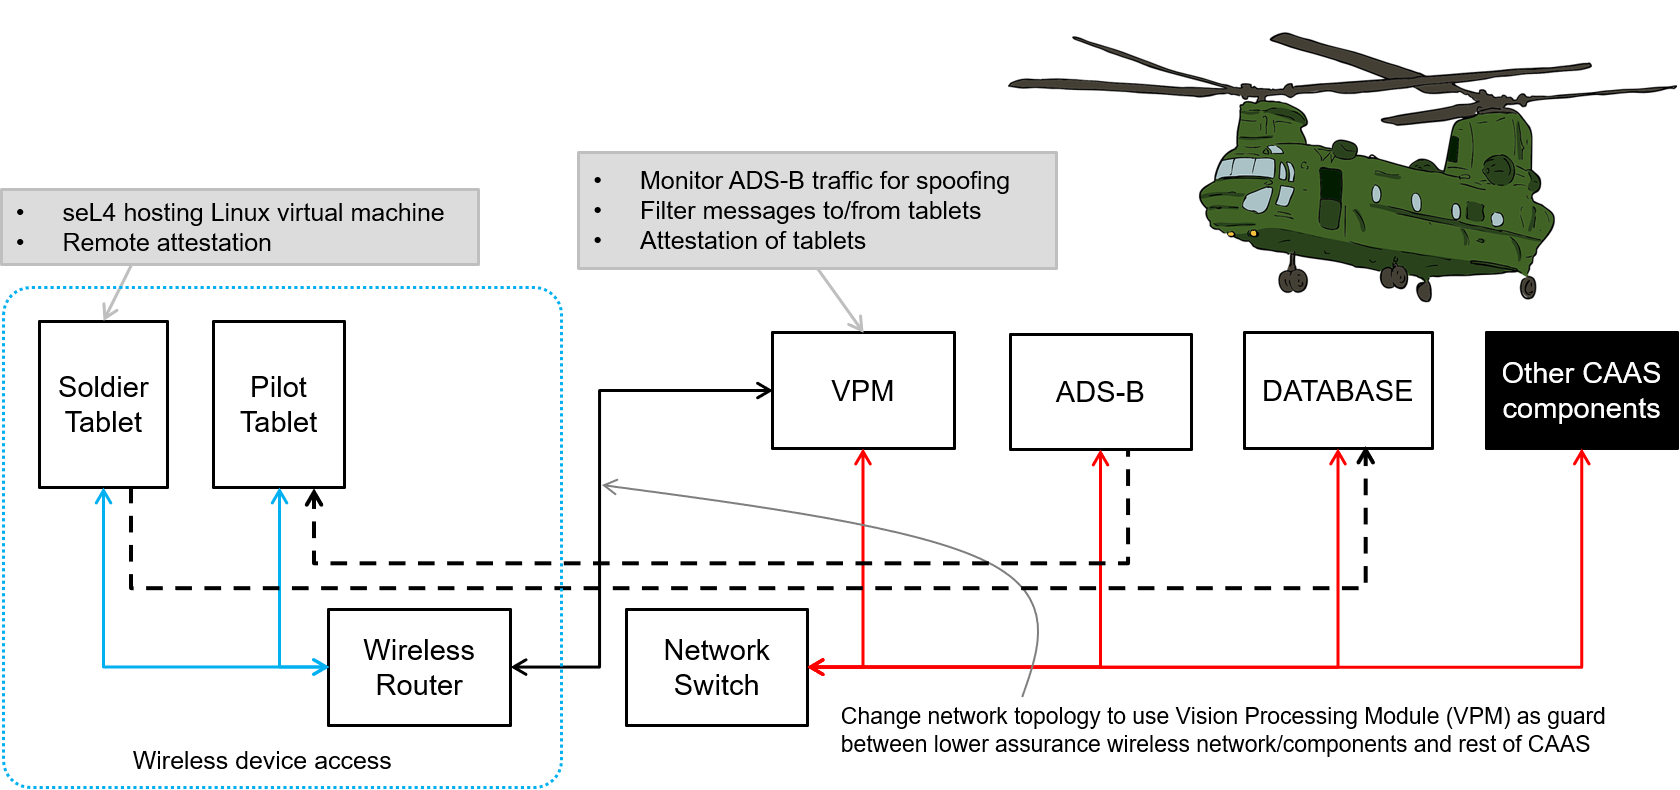
\includegraphics[width=\textwidth]{./figs/caas-arch.png}
        \end{center}
	\caption{Cyber-resilient software architecture adding wireless device access to CH-47 avionics.} 
	\label{fig:caas-arch} 
\end{figure*}

The CH-47F demonstration system
for CASE focused on integrating pilot and soldier wireless tablet computers for
increased situational awareness and display of Automatic Dependent Surveillance-Broadcast (ADS-B)
data regarding nearby air traffic (\figref{fig:caas-arch}).  
BriefCASE tools were used to implement this networking enhancement while ensuring that no new cybersecurity
vulnerabilities were introduced.  A high-assurance gateway was added between the existing CAAS 
network and the new wireless network, including new components for monitoring messages to and from the wireless 
devices.  Remote attestation was also added to ensure that any devices that attempt to join the wireless network
are running trustworthy software.   
This also required porting the seL4 microkernel to an existing CAAS
processing module (the vision processing module, or VPM) that would be repurposed to serve as the secure gateway.  

%This vision processing module, or VPM, is provisioned to allow only vetted
%traffic to/from the aforementioned wireless clients in order to provide situational awareness data
%to pilots and soldiers, as well as to provide a platform for the execution of CASE-tool-generated
%filters, monitors, attestation gates, etc.

The CAAS engineers first developed an AADL model of the CH-47F CAAS system. They added the
enhanced capabilities for wireless access described above, resulting in a baseline architecture. The 
engineers then analyzed their baseline AADL architecture utilizing the GearCASE and DCRYPPS tools,
resulting in a set of cyber requirements. They employed the BriefCASE AADL tools to add
filters, monitors, attestation gates, and seL4 isolation to satisfy the cyber
requirements. ADS-B anti-spoofing monitors were also developed by the CAAS team to 
detect inconsistencies in aircraft position and velocity trends,
bad traffic identifiers, and other possible indicators of spoofed aircraft.

The specifications for the filters and monitors were developed by the CAAS engineers
using the AGREE contract language, with assistance from our research team.  The SPLAT tool was
used to synthesize the monitors and filters from the AGREE specifications
with high assurance, as described above. The HAMR tool was then used
to generate infrastructure code for the overall system running on seL4.
%including the seL4 CAmkES components, CAmkES I/O, the processing schedule, etc.

The tablet operating environment was modified to run application software in a Linux virtual machine
hosted on seL4.  This was necessary to add the remote attestation components.  

%utilized either an off-the-shelf Android environment, or a Linux
%guest OS running on seL4. This provided the CASE remote attestation team with differing challenges
%when it came to the measurement and attestation of the tablet platform types, and provided the CASE
%independent evaluators a variety of options for formulating attacks against the system. The ADS-B
%anti-spoofing monitor developed by the CAAS team detected position/velocity trend inconsistencies,
%duplicate traffic identifiers, as well as ``teleporting'' aircraft.

The port of the seL4 microkernel to the VPM was complicated by the need for network
proxy and adapter components to bridge the untrusted wireless network to the rest of the sytem in a trustworthy
manner, including the ability to filter encrypted network traffic payloads. Fortunately, dedicated
processing cores were available on the VPM for the provisioning of these ``low-side'' and ``high-side''
components. This code had to be manually written due to the complexity of dealing with
off-the-shelf networking technologies.  Automating the synthesis of network adapter and proxy components
is future work.

As initial users of the BriefCASE tools, the CAAS engineers encountered some limitations in the
specification expressiveness and documentation, as might be
expected for the first use of a research tool suite by product area developers. 
This led to improvements in the tools to add or extend capabilities.  Initial estimates of
processing time required the complex monitoring components turned out to be optimistic,
requiring an optimization effort. Lack of detailed seL4 support for the target hardware led to more
extensive porting efforts for the VPM and tablets than was originally anticipated, and tablet
hardware instabilities further hampered the porting effort. But all in all, the CASE tools were able
to be productively used by Collins product area engineers to produce the CH-47F CAAS demonstration
system on time and within budget, providing our research team with valuable feedback on the
strengths and weaknesses of the current BriefCASE tool envionment.
